\documentclass[11pt,a4paper]{rapport-stage-umons}

\usepackage[utf8]{inputenc}
\usepackage[T1]{fontenc}
\usepackage[francais]{babel}

\usepackage{graphicx}
\usepackage{verbatim}

\title{4 mois à Paris au sein de Be Sport et Ocsigen}
\author{Danny \textsc{Willems}}
\date{2016--2017}
\directeur{Christophe \textsc{Troestler}}
\maitre{Vincent \textsc{Balat}}
\discipline{Mathématiques}
\institut{Département de mathématiques}

\usepackage{amssymb,amsmath,amsthm}
\usepackage{hyperref}% hyperliens dans le PDF, pas pour impression
\usepackage{xcolor}

\usepackage{listings}
\usepackage{courier}
\lstset{basicstyle=\footnotesize\ttfamily, breaklines=true}

\lstset{
  framexleftmargin=16pt,
  frame=tb,
  framerule=0pt
}

%%%%%%%%%%%%%%%%%%%%%%%%%%%%%%%%%%%%%%%%%%%%%%%%%%%%%%%%%%%%%%%%%%%%%%%%
%% Vos macros


%%%%%%%%%%%%%%%%%%%%%%%%%%%%%%%%%%%%%%%%%%%%%%%%%%%%%%%%%%%%%%%%%%%%%%%%

% Compile uniquement certains morceaux sans perdre les références
% automatiques et la table des matières des parties déjà compilées :
%\includeonly{introduction,chapitre1}

\begin{document}
% Éventuellement utiliser l'environnement « preface » pour avoir une
% numérotation des pages en chiffres romains.

\tableofcontents

\section{Présentation de l'entreprise}

\subsection{Be Sport}

Be Sport\cite{besport} est une entreprise française développant un réseau social
et un média centrés sur le sport. Initialement lancé en 2012 à San Francisco
aux États-Unis, Be Sport s'est implanté à Paris fin 2015 sous la
direction de Philippe Robert, principal investisseur, et de membres de l'équipe d'Ocsigen.

Contrairement à la grande majorité des plateformes du sport qui se concentrent
sur les professionnels, Be Sport est une plateforme regroupant tous les
types d'acteurs du sport: amateurs, professionnels, clubs, fédérations, médias,
etc.

Avec Be Sport, il est possible de

\begin{itemize}
  \item suivre des sportifs, amateurs comme professionnels, des clubs et des
    fédérations ;
  \item se connecter avec d'autres personnes inscrites sur la plateforme ;
  \item créer des événements sportifs (par exemple des tournois, des concours,
    des championnats) et inviter ses connexions ;
  \item discuter grâce à un tchat ;
  \item suivre les dernières nouvelles des sports qui nous intéressent ;
  \item partager des nouvelles, des résultats ;
  \item et bien plus : de nouvelles fonctionnalités sont ajoutées très régulièrement.
\end{itemize}

Le trait de Be Sport qui m'a attiré pour le choix de mon stage est la
technologie utilisée: OCaml et en particulier le framework web Ocsigen.

\subsection{Ocsigen}

Ocsigen\cite{ocsigen-website} est le plus connu des frameworks web écrit en
OCaml.

Lancé en fin d'année 2004 par Vincent Balat, Ocsigen\footnote{Pour \og OCaml site
  generator \fg.} souhaite apporter des solutions, innovantes à ses débuts, à
plusieurs problématiques du développement d'applications web:

\begin{enumerate}
  \item utiliser un seul et unique langage (OCaml) pour développer la partie cliente et
    la partie serveur. En effet, la plupart des architectures utilisent deux
    langages différents. Cela implique qu'un développeur web doit apprendre différents
    langages. Du coté de l'entreprise, cela peut aussi impliquer de devoir
    embaucher deux développeurs: un pour le coté client, souvent appelé
    \og développeur front-end \fg, et un autre pour le coté serveur, souvent appelé
    \og développeur back-end \fg.
  \item pouvoir, dans un seul fichier, décrire les morceaux de code qui seront
exécutés coté client et ceux qui seront exécutés coté serveur. Ceci est réalisé
à travers une extension de syntaxe PPX d'OCaml\footnote{Gabriel Radanne, aka
  Drup, travaille sur un compilateur Eliom, voir
  \cite{ocsigen-eliomlang-github}. Ce compilateur fournit plus de possibilités
  que PPX.}.
  \item permettre d'injecter du code serveur dans la partie cliente.
    L'utilité de cette fonctionnalité est de laisser le serveur évaluer
des expressions pour décharger le client de certains calculs qui pourraient être
lourds.
  \item typer statiquement (au moment de la compilation, non à l'exécution), les
    programmes (coté serveur et coté client) ainsi que le code injecté.
  \item pouvoir utiliser les bibliothèques du langage de base (OCaml), que cela
    soit coté client ou coté serveur.
\end{enumerate}

Bien que la plupart des points soient résolus indépendemment par plusieurs
technologies (Node.js\cite{nodejs-website}, Meteor\cite{meteor-website},
Scala\cite{scala-website} + Play\cite{play-website} +
ScalaJS\cite{scalajs-website}, entre autres), aucune technologie unique, à ma
connaissance, répond à tous les besoins.

Le projet Ocsigen répond à chacun de ces besoins, et même plus. Le projet est
composé de plusieurs sous projets dont

\begin{itemize}
  \item Ocsigen Server\cite{ocsigen-server-github}, un serveur web écrit entièrement en OCaml.
  \item un compilateur de bytecode OCaml vers JavaScript, js\_of\_ocaml\cite{ocsigen-js-of-ocaml-github}, qui
    pemet d'écrire du code OCaml et de l'exécuter dans le navigateur web. En
plus du compilateur, js\_of\_ocaml fournit un binding OCaml assez complet (bien
que bas-niveau) au DOM et à la librairie standard JavaScript. Une particularité
de js\_of\_ocaml comparé à d'autres compilateurs/transpileurs OCaml vers
JavaScript est le support de tout le langage OCaml, sans syntaxe particulière.
  \item une bibliothèque implémentant le standard XML de manière typée en OCaml,
TyXML\cite{ocsigen-tyxml-github}. Cela permet d'écrire en particulier de l'HTML
typé et de respecter ainsi les normes W3C.
  \item Eliom, qui permet d'écrire, avec un haut niveau
    d'abstraction et des concepts innovants, des applications web
client-serveur. Eliom dépend de Ocsigen Server, TyXML et js\_of\_ocaml et
fournit une abstraction plus haut niveau des API de ces différents projets.
  \item Ocsigen Toolkit, un ensemble de widgets web (différents boutons, des
    menus, des icones de chargements, etc) permettant d'utiliser les
    particularités d'exécution client-serveur d'Eliom.
  \item Ocsigen Start qui fournit un template Eliom avec un ensemble de
    bibliothèques pour gérer des utilisateurs, des groupes d'utilisateurs, des
    notifications push, etc. Ocsigen Start permet également de développer des
    applications mobiles, le tout en OCaml.
\end{itemize}

Ayant passé beaucoup de temps à apprendre et à travailler sur Eliom et Ocsigen
Start, l'apprentissage et la maitrise de ces deux bibliothèques ont eu une
grande importance lors de mon stage. 

\subsubsection{Eliom}

Le but principal d'Ocsigen est d'unifier le développement de la partie serveur
et la partie cliente en utilisant un langage unique et typé statiquement.

Eliom est le centre du projet Ocsigen (avec comme dépendances Ocsigen Server et
js\_of\_ocaml) et constitue la solution aux besoins donnés ci-dessus.
Eliom fournit également une interface de haut
niveau pour des besoins usuels en programmation web comme un système de
notifications (\verb|Eliom_notif|), de création d'HTML réactif
(\verb|Eliom_shared.React.S|) et des données réactives
(\verb|Eliom_shared.ReactiveData|), d'échange de données entre clients
(\verb|Eliom_bus|), de créations de services pour les routes de l'application et
des enregistrements de ces services (\verb|Eliom_service| et
\verb|Eliom_registration|), un système de gestion de cookies
(\verb|Eliom_cookies|), création de formulaires typés
(\verb|Eliom_form|), un système de RPC (en utilisant la fonction \\
\verb|Eliom_client.server_function|) et bien plus.

De plus, depuis Eliom 6, il est possible d'écrire des applications mobiles.

En utilisant PPX, Eliom ajoute de la syntaxe au langage OCaml usuel.\footnote{Pour plus
d'informations sur le langage Eliom, voir \cite{gabriel-radanne-paper-eliom}.}
Eliom fournit également des outils pour simplifier la compilation:
\begin{itemize}
  \item \verb|eliomc| pour compiler du code serveur en bytecode.
  \item \verb|eliomopt| pour compiler du code serveur en natif.
  \item \verb|js_of_eliom| pour compiler en JavaScript le code client.
\end{itemize}

Pour différentier les fichiers contenant du code Eliom et ceux qui n'en \\
contiennent pas, de nouvelles extensions de fichiers sont utilisées: \verb|eliomi|
pour l'équivalent de \verb|mli| et \verb|eliom| pour \verb|ml|.

Pour définir une expression qui sera évaluée coté serveur (resp. coté client), la syntaxe
\verb|let%server v = 42| (resp. \verb|let%client v = 42|) est utilisée. Il
existe aussi la syntaxe \verb|let%shared v = 42| pour définir en même temps une
même expression coté client et coté serveur. L'équipe d'Ocsigen travaille
également sur un nouveau compilateur Eliom, voir
\cite{ocsigen-eliomlang-github}, qui fournit, entre autres, la même extension
pour les types (\verb|type%server t = int|) et le langage de modules
(\verb|module%server M = struct type t = int end|), non disponibles actuellement avec PPX.

Il est également possible de définir des valeurs coté serveur et d'y accéder
coté client avec la syntaxe \verb|let%client v = ~%server_value| où \\
\verb|server_value| est une valeur définie coté serveur.

Une dernière possibilité avec Eliom est, à l'inverse d'évaluer une expression
coté serveur et la récupérer coté client, il est possible, dans une expression
coté serveur, de calculer une expression coté client et d'en récupérer le
résultat coté serveur.
La syntaxe utilisée est \verb|let%server x = [%client 5 + 2]|.

Si plusieurs xpressions doivent être évaluées coté serveur (resp. coté client),
il est possible d'utiliser la syntaxe \verb|[%%server expressions]| (resp. \\
\verb|[%%client expressions]|) dans les fichiers \verb|eliom| et la syntaxe \\
\verb|[%%server.start] expressions| (resp. \\ \verb|[%%client.start] expressions|)
dans les fichiers \verb|eliomi|.

\subsubsection{Ocsigen Start}

Anciennement eliom-base-app\footnote{Le nom fut changé pendant la période de
  mon stage.}, le projet Ocsigen Start\cite{ocsigen-start-github} est la base de
l'application Be Sport, distribué sur GitHub sous licence LGPL.

A travers ce projet, l'équipe d'Ocsigen souhaite fournir un ensemble de
fonctions permettant de créer très facilement un prototype d'une application web
et mobile. Cela implique, en partie, de gérer très facilement une base de
données d'utilisateurs, de groupes, d'emails, fournir des services usuels
(inscriptions d'utilisateurs, envoi d'email de confirmation, connexion,
modification de données personnelles), permettre de gérer plusieurs emails par
utilisateurs, le redimensionnement et cropping de photos et fournir des systèmes
de sessions et de cache.

En plus de la bibliothèque, Ocsigen Start fournit un un template qui montre
comment utiliser les diverses fonctionnalités d'Eliom comme les
RPC\footnote{Remote Procedure Calls}, les notifications à travers
\verb|Eliom_notif| mais aussi les fonctions de la bibliothèque.

Le template fourni permet également d'avoir une application mobile (Android,
iOS, Windows Phone) de l'application web développée. Le framework web et mobile
Cordova est utilisé pour l'application Android et iOS tandis que le concept
d'Universal Web App est utilisée pour Windows Phone\footnote{Ceci en raison de
  la faible compatibilité des plugins Cordova sous Windows Phone.}.

Ocsigen Start réalise des choix pour les développeurs comme PostgreSQL ou SASS
(pré-processeur CSS).
Dans les prochaines versions, Ocsigen Start devrait être compatible avec
différents gestionnaires de bases de données comme MySQL.
\section{Tâches effectuées}

Durant mon stage, j'ai réalisé différentes tâches touchant à différents
domaines. Ces tâches, j'ai eu la liberté de les choisir (en fonction des besoins
de Be Sport et de la répartition de celles-ci) au fur et à mesure des quatres
mois passés chez Be Sport. Certaines tâches, que je qualifierai de mineures et
majoritairement dans Ocsigen Start, étaient ajoutées aux tâches principales.

Pendant tout mon stage, je n'ai jamais contribué directement au code de la
plateforme Be Sport: le travail que j'effectuais était principalement dans Ocsigen Start
(que Be Sport utilise comme base) ou dans un projet séparé (comme pour les
notifications push) et celui-ci était utilisé par un développeur de Be Sport comme
base. Cette méthode a été choisie par Vincent Balat pour que je puisse être
productif plus rapidement car sinon, j'aurais du, en plus du projet Ocsigen qui
est déjà assez conséquent, comprendre l'ensemble de Be Sport.

\subsection{OAuth2.0 et OpenID Connect}

Lorsque je suis arrivé le premier jour, j'ai pu choisir une première tâche dans
une liste de prochaines fonctionnalités devant être développées dans Be Sport.

J'ai choisi l'implémentation d'un système semblable à Facebook
Login\cite{facebook-login} dans Be Sport, appelée Be Sport Connect\footnote{La dénomination n'a pas été officiellement
  choisie mais celle-ci était utilisée pour parler de cette fonctionnalité.}.
Cette fonctionnalité doit permettre à des applications indépendantes de Be Sport
de pouvoir utiliser un compte créé sur Be Sport sans que l'utilisateur donne, à
nouveau, certaines informations comme son adresse email, son nom, son prénom et
un mot de passe et sans pour autant accéder à
toutes les données possédées par Be Sport sur l'utilisateur (comme certains
sites font avec Facebook, LinkedIn, Twitter ou encore GitHub).\footnote{Par la
suite, les
  priorités de Be Sport ont changé
  et j'ai donc laissé de côté cette partie pour me focaliser sur Ocsigen Start
  et les notifications push, tâches décrites ci-dessous. Vers la fin de mon
  stage, le travail a été repris pour mettre à jour avec les changements
  d'Ocsigen Start. Cependant, l'implémentation, bien que très avancée, n'est pas
encore finie.}.
L'idée derrière cette fonctionnalité est de séparer l'application Be Sport en
plusieurs applications indépendantes. Par exemple, le tchat Be Sport, actuellement
dépendant de Be Sport, pourrait être une application entièrement séparée de Be
Sport sous le nom de \emph{Be Sport Chat}. Un autre exemple est une application
\emph{Be Sport Location} qui permet de localiser un utilisateur connecté et
lister les différents événements proches de lui. Ces deux applications ont
besoin de créer des comptes pour retenir diverses informations, d'où l'intérêt
de Be Sport Connect pour éviter de devoir créer des comptes séparés pour les
deux applications en plus de Be Sport.


\subsection{JWT : Json Web Token}

Comme dit précédemment, OpenID Connect utilise le standard JWT (Json Web
Token)\cite{official-jwt-website, official-openid-connect-website, rfc-jwt}
pour représenter de manière sécurisée des demandes (\textbf{claims} en anglais) et les
transférer entre deux applications en utilisant des \textit{jetons} (ou
\textit{token} en anglais).
Aucune bibliothèque n'existant en OCaml pour gérer ce standard, j'ai du
l'implémenter. La bibliothèque est disponible sur le GitHub de Be
Sport\cite{ocaml-jwt-github} ainsi que
dans OPAM sous le nom \emph{jwt} et est distribué sous licence LGPL.

Un JSON Web Token est une chaine de caractères composé de trois éléments séparés
par des points:
\begin{itemize}
  \item un \textit{header} comprenant le type du jeton (dans notre cas
    \emph{JWT}) et l'algorithme de chiffrement (par exemple
    \emph{HMAC-SHA-256}, identifié par \\ \emph{HS256})
    représenté par un JSON. Le premier élément du JSON Web Token est le
    résultat de ce JSON en utilisant l'encodage base64\cite{rfc-base64}.
  \item les \textit{claims} ou le \textit{payload} comprenant les demandes ou
    des méta données devant être transférées. Le résultat est aussi représenté
    par un JSON encodé en utilisant l'encodage base64.
  \item la \textit{signature} qui fournit à ce standard un niveau de sécurité
    pour la transmission des données. Elle consiste en le résultat du chiffrement
    (par l'algorithme de chiffrement donné dans le header) de la concaténation des
    deux encodages base64 précédents séparés par un point. Si l'algorithme de
    chiffrement utilisé est \emph{HS256}, une clef secrète est utilisée pour
    chiffrer. La chaîne de caractères résultante du chiffrage est encodée en
    utilisant l'encodage base64 et représentera le dernier élément du jeton.
\end{itemize}

\begin{figure}
  \centering
  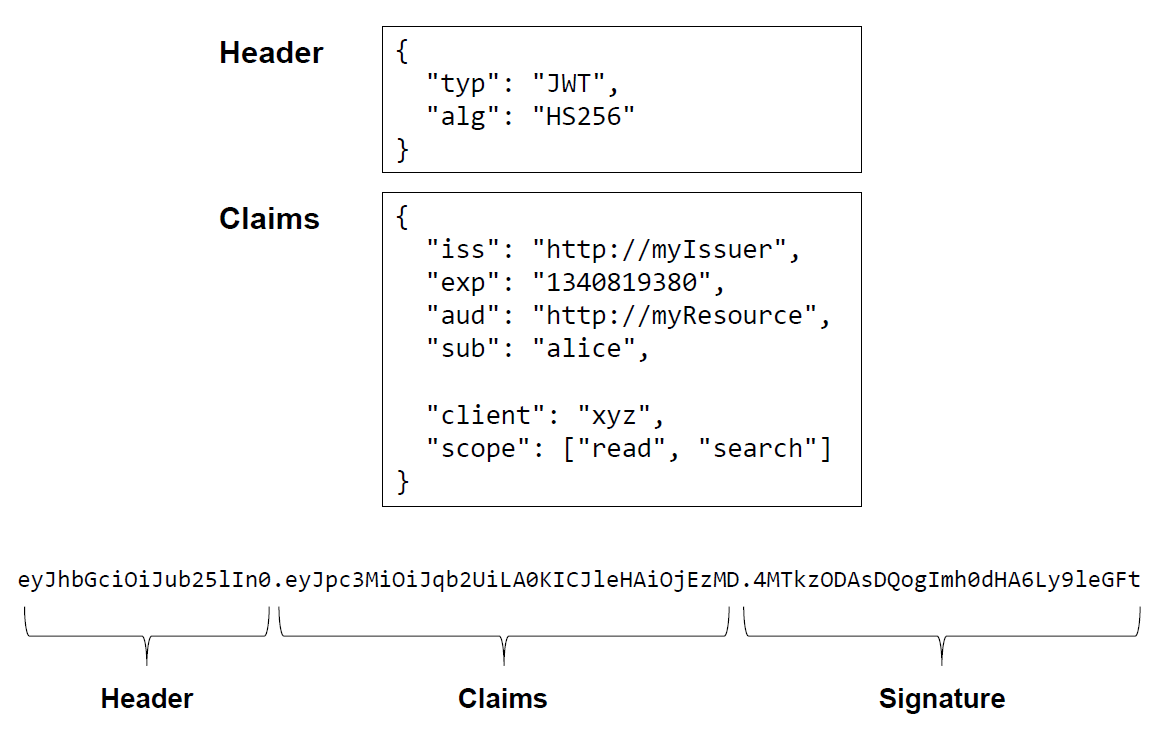
\includegraphics[width=300px]{jwt-example.png}
  \caption{Schéma expliquant la structure d'un JSON Web Token. Le jeton qui sera
    échangé entre les deux applications est la chaîne de caractère. Les parties header
    et claims résultent de l'encodage base64 des JSON respectifs. La signature
    est générée grâce à l'algorithme HS256 en utilisant une clef secrète qui
    n'est pas donnée dans ce cas.}
\end{figure}

Un exemple complet est donné sur le site officiel du standard\cite{official-jwt-website}.

La bibliothèque OCaml \emph{jwt}\cite{ocaml-jwt-github} fournit une interface
simple pour créer, chiffrer et déchiffrer un JWT.

Un token est représenté par un type abstrait \verb|t|. Le token chiffré peut
être généré grâce à la fonction \verb|token_of_t|. Le header et les différents
claims peuvent être reconstitués en JSON en utilisant la fonction
\verb|t_of_token|.

Au niveau des algorithmes de chiffrement,
\textit{Cryptokit}\cite{ocaml-cryptokit-ocaml-forge} est utilisé et uniquement
HS256 est supporté\footnote{Car uniquement cette méthode est utilisée pour OpenID
  Connect}. Les différents algorithmes sont contenus dans un type somme \verb|algorithm|.

Un header est représenté par un type abstrait \verb|header| et une valeur de ce
type peut être créé grâce à la fonction \verb|header_of_algorithm_and_type|.

Une claim est représentée par un type abstrait \verb|claim| et une liste de
claim usuel sont déjà définis (comme \emph{iss}, \emph{sub} et \emph{exp} qui
sont utilisés dans OpenID Connect). De nouveau claims peuvent être créées en
utilisant la fonction \verb|claim| qui prend le nom en paramètre. 

Le payload, c'est-à-dire l'ensemble des claims, peut être créé à travers la
valeur \verb|empty_payload| et la fonction \verb|add_claim|.
Pour obtenir les différentes claims d'un payload, la fonction \verb|find_claim|
peut être utilisée.

\subsection{Récupération de données, json2ical et binding à \\ Node.js  et Nightmare}

Comme expliqué dans la présentation de Be Sport, l'application permet d'accéder
à toutes les nouvelles des sports qui vous intéressent comme les résultats des
derniers matches ou les prochaines compétitions ou tournois.
Afin de fournir le plus de nouvelles à ses utilisateurs, Be Sport récupère les
données de différents sites comme \href{https://eurosport.fr}{Eurosport} pour le
football ou \href{https://atpworldtour.com}{atpworldtour} pour le tennis.
Cette tâche nécessite d'analyser comment le site visé fonctionne et automatiser
la visualisation des données souhaitées.

Dans les premiers jours, il m'a été demandé de récupérer les résultats provenant
du site \verb|www.atpworldtour.com|.
Une première version stable a été écrite à l'aide de JavaScript et de
Nightmare\cite{nightmare-website}. Cette version exportait les données vers un
format JSON. Cependant, le format demandé par Be Sport était
iCalendar avec des champs spécifiques.
Un match, une compétition ou un résultat est représenté par un événement
iCalendar (composant \verb|VEVENT|) et possède obligatoirement un ID. Les
matches sont représentés comme des sous-événements des compétitions et
possèdent, dans le format iCalendar, un champ supplémentaire
(\verb|X-PARENT-ID|) afin de pouvoir retrouver la compétition dont les matches
proviennent.

\subsubsection*{json2ical}

Après avoir remarqué que d'autres scripts utilisés pour récupérer les données
d'autres sites travaillaient d'abord en JSON pour ensuite convertir au format
iCalendar, j'ai décidé d'écrire une bibliothèque, \emph{json2ical}, qui permet
de convertir un fichier donné au format JSON dans le format iCalendar.
Cette bibliothèque, écrite en JavaScript avec Node.js, exporte une unique
fonction, \verb|json_to_ical| qui prend en paramètre:

\begin{itemize}
  \item un objet JavaScript (représentant le JSON).
  \item (optionnel) un ensemble de clef-valeur permettant de définir comment les champs JSON
    vont être convertis dans le format iCalendar. Par défaut, chaque champ du
    JSON est préfixé par \verb|X-| (norme utilisée pour Be Sport). Dans tous les
    cas, le nom du champ est mis en majuscule.
  \item (optionnel) un entier représentant l'ID du premier événement.
\end{itemize}

Par exemple, avec la configuration par défaut,

\begin{lstlisting}
  {
    "summary": "Hello Be Sport",
    "start": 2048,
    "finish": 4096
  }
\end{lstlisting}

sera transformé en

\begin{lstlisting}
    BEGIN:VEVENT
    X-SUMMARY:Hello Be Sport
    X-START:2048
    X-FINISH:4096
    X-ID:1
    END:VEVENT
\end{lstlisting}

et avec la configuration

\begin{lstlisting}
  {
    "title": "summary",
    "begin": "dtstart",
    "end": "dtend"
  }
\end{lstlisting}

cela donnera

\begin{lstlisting}
  BEGIN:VEVENT
  SUMMARY:Hello BeSport
  DTSTART:2048
  DTEND:4096
  X-ID:1
  END:VEVENT
\end{lstlisting}

pour le JSON initial
\begin{lstlisting}
  {
    "title": "Hello BeSport",
    "begin": "2048",
    "end": "4096"
  }
\end{lstlisting}

\subsubsection*{Binding à Node.js et Nightmare}

Un autre stagiaire présent, Omar Chebib, a aussi du réaliser un script pour
récupérer des données sur \href{https://eurosport.com}{Eurosport} avec
JavaScript et Nightmare. Nous avons tous les deux remarqué qu'il nous était
très difficile de déboguer et d'avoir un script robuste sans le typage statique
d'OCaml.

Pendant deux journées, nous avons alors pris l'initiative de réaliser une deuxième version de
nos scripts respectifs en utilisant cette fois-ci OCaml et le compilateur
\emph{js\_of\_ocaml}. Pour cela,
nous avons écrit un binding haut niveau vers Node.js et Nightmare en utilisant
\emph{gen\_js\_api}\cite{gen-js-api-github}.

Les bindings\cite{besport-ocaml-node-github,
  besport-ocaml-node-nightmare-github} sont disponibles sur le GitHub de Be Sport sous licence
LGPL. Bien que partiels,
ceux-ci sont fonctionnels et nous ont permis d'améliorer notre productivité.

\subsubsection*{Interface OCaml pour l'importation dans la base de données}

Egalement avec Omar Chebib, après avoir fini notre script de récupération de
données, il nous a été demandé d'importer les données dans la base de données de
Be Sport. Les données récupérées comprennent les championnats, le nom des
équipes ainsi que le nom des joueurs et doivent être importées selon un schéma
de tables bien définies. Chaque site a ses propres tables.

A la place de réaliser un script d'importation pour chaque site, nous avons une
nouvelle fois pris l'initiative d'écrire une interface générique par sport.
Par exemple, pour le football, les données devant être récupérées sont le plus
souvent dans le même format:
\begin{itemize}
  \item un événement parent représentant le championnat.
  \item des sous-événements représentant les matches.
  \item pour chaque match, le nom des équipes, le résultat, les joueurs, les
    buts, les cartes jaunes et rouges.
\end{itemize}

Nous avons écrit une bibliothèque OCaml et un binaire abstrayant les
données.
Sur la plupart des sites, les scripts récupèrent les données par matches afin de
pouvoir en récupérer plusieurs en parallèle et ainsi accélérer l'ensemble
du processus. La
bibliothèque fournit un type \verb|Fixture.t| comprenant toutes les informations
relative à un match et est utilisée avec le binding à
Nightmare et est compilée en JavaScript pour récupérer les données. Une fonction
\verb|Fixture.t_to_js| donne la représentation JavaScript devant être
utilisée pour l'importation. Cette représentation JavaScript est alors écrite
dans un fichier au format JSON.

Le binaire, nommé \verb|bs-import|, prend en paramètre le JSON précédent et se charge d'importer l'ensemble des données dans la base de données.

Au final, le procédé de récupération fonctionne de la manière suivante:

\begin{enumerate}
\item Analyse du site.
\item Utilisation du binding à Nightmare pour accéder aux données.
  \item Abstraction des données d'un match à travers le type \verb|Fixture.t| et
    exportation dans un fichier au format JSON.
\end{enumerate}

Et l'importation de données se résume en l'utilisation du binaire de la manière
suivante:

\verb|bs-import [nom_du_championnat] -f [fichier_json]|.

Cette dernière version permet de se focaliser uniquement sur le parsing du site
web et non sur la représentation des données ou encore de l'importation dans la
base de données.
De plus, pour permettre la récupération de données d'autres sports, il suffit
d'écrire le type OCaml correspondant, la fonction exportant en JSON et les
fonctions travaillant sur la base de données.

\subsection{Ocsigen Start}

A partir de la huitième semaine, il m'a été demandé de travailler uniquement sur
Ocsigen Start et ce jusqu'à la fin de mon stage.

Beaucoup de personnes ont travaillé sur Ocsigen Start. Cependant, à
travers l'évolution des fonctionnalités et l'ajout de nouvelles, aucune analyse
n'avait été réalisée pour supprimer les fichiers ou fonctions inutiles ou encore
réorganiser le code pour éviter la duplication.

Après avoir analysé la bibliothèque et le fonctionnement du template dans son
ensemble, j'ai effectué un premier nettoyage et une première réorganisation du
code. Cela a permis de remarquer qu'une partie des fichiers de l'application
mobile était inutile et alourdissait l'installateur résultant.

\subsubsection*{Tâches mineures}

Une partie du travail réalisé sur Ocsigen Start consistait en des tâches prenant
quelques heures à quelques jours pour certaines. En voici une liste,
non-exhaustive:

\begin{itemize}
\item Réorganisation des Makefiles. Le template d'Ocsigen Start fonctionne avec
  des Makefiles pour l'ensemble du processus de compilation. J'ai choisi de
  déplacer toute la configuration du template dans un Makefile
  \verb|Makefile.options|, déplacer les cibles relatives à la base de données
  dans un Makefile \verb|Makefile.db|, épurer les makefiles de cibles superflues
  ou plus utilisées.

  \item Permettre l'utilisation de SASS comme pré-processeur CSS. En résulte un
    nouveau Makefile relatif au style s'appelant \verb|Makefile.style| et une
    option \verb|USE_SASS| qui permet de choisir ou non d'utiliser SASS.
  \item Suppression de la dépendance à Ocsigen Widgets, ancêtre de Ocsigen Toolkit.
  \item Utilisation du bon binaire \verb|pg_ctl| pour PostgreSQL sur Debian. Le
    binaire \verb|pg_ctl| permet de gérer PostgreSQL et le chemin vers celui-ci
    est différent que l'on soit sous Debian, Ubuntu ou Mac OSX.
  \item Compatibilité des Makefiles au niveau des utilitaires BSD et GNU.
    L'implémentation de certains binaires usuels comme \verb|sed| ou \verb|find|
    est différente entre ceux fournis par défaut sur Mac OSX ou sur une
    distribution GNU/Linux. Il m'a fallu rendre les Makefiles compatibles avec
    BSD car ils ne l'étaient pas défaut et il était donc impossible d'utiliser
    le template sur une machine disposant des outils BSD.
  \item Remise en place de l'intégration continue avec Travis. Depuis quelques
    mois, voire quelques années, l'intégration continue ne fonctionnait pas et
    des emails étaient envoyés à chaque commit sur le dépot GitHub.
  \item API de la bibliothèque. Une très grande partie de la bibliothèque
    d'Ocsigen Start n'était pas documenté: j'ai alors passé plusieurs jours à la
    documenter. Cela m'a permis d'avoir une vue plus globale sur tout le projet.
  \item Utilisation des section \verb|let%section| à la place des blocs
    \verb|[%%section.start]| et \verb|[%%section expr]|. L'utilisation de
    \verb|let%section| rend le code plus lisible.
  \item Suppression de la dépendance au binding à ImageMagick. Une seule
    fonction dans le module \verb|Os_uploader| utilisait le binding pour la
    sélection d'une partie d'une photo. La nouvelle solution proposée utilise
    directement la ligne de commande \verb|convert|.
  \item Style CSS de la gestion de plusieurs emails dans les préférences
    utilisateurs.
\end{itemize}

\subsubsection*{Notifications push}

Les notifications push sont des messages envoyés par le serveur (appelé alors
\emph{serveur push}) à un client.
Il est très courant de voir des notifications push sur les systèmes Android
et iOS comme celles de Facebook, Twitter, ou encore les mises à jour des
applications du Play Store.

\begin{figure}
  \centering
  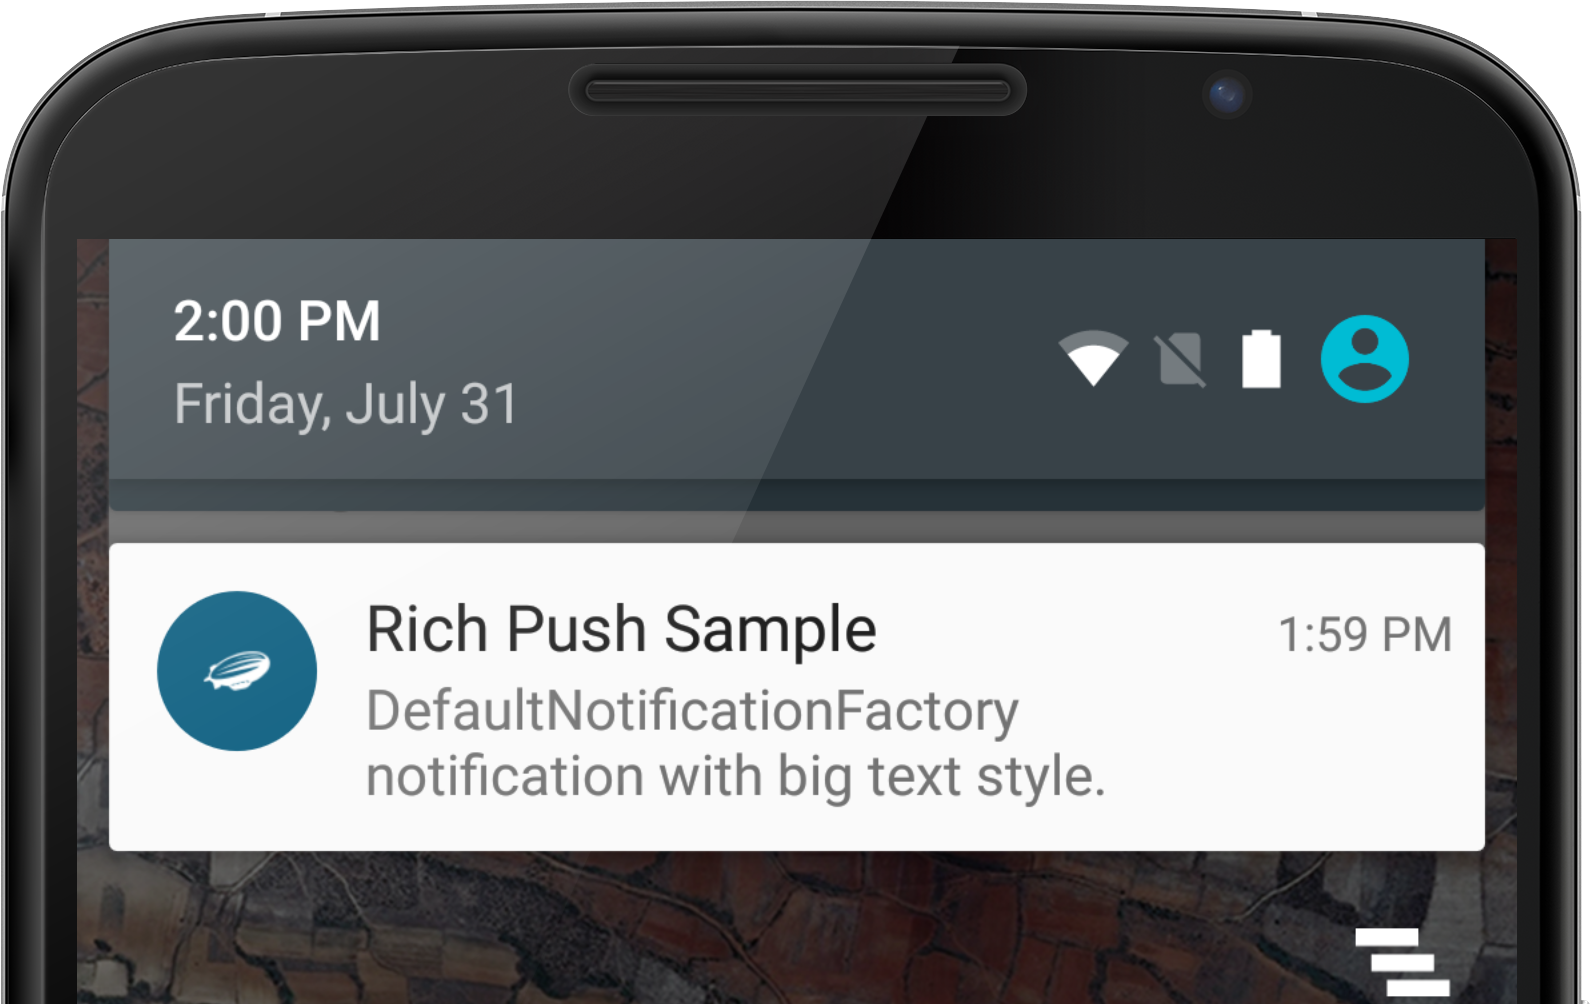
\includegraphics[height=100px]{push-notification-example-android.png}
  \caption{Exemple de notification push sur Android.}
\end{figure}

D'un point de vue business et croissance, les notifications push
augmentent la rétention des utilisateurs car elles motivent l'utilisateur à
accéder à l'application.

Tout en travaillant sur Ocsigen Start en général, il m'a été demandé de
réfléchir à un système de notifications push pour l'application Be Sport, et de
manière plus général, pour le projet Ocsigen Start.

Bien qu'il soit possible de créer un serveur push,
il est recommandé, pour des raisons de sécurité, de maintenance et de communauté
d'utiliser un service de notifications push existant.

Les systèmes d'exploitations mobiles les plus connus possèdent chacun leur propre
service de notifications push:
\begin{itemize}
  \item Google - Firebase Cloud Messaging (\emph{FCM}), anciennement Google Cloud
  Messaging (\emph{GCM}).
  \item Apple - Apple Push Notifications service (\emph{APNs}).
  \item Microsoft - Windows Push Notifications Services (\emph{WNS}).
\end{itemize}

Après avoir analysé les différentes solutions disponibles, je me suis orienté
vers FCM pour les raisons suivantes:

\begin{enumerate}
  \item beaucoup d'applications l'utilisent depuis longtemps.
  \item l'interface pour envoyer des notifications est simple: une URL à
    laquelle il faut envoyer les données de la notification au format JSON.
  \item il est possible, avec la même interface, d'envoyer les notifications sur
    Android et iOS, ce qui rend unique FCM par rapport aux autres services cités.
  \item il existe un plugin Cordova, \emph{phonegap-plugin-push}.
  \item j'avais déjà réalisé un binding OCaml au plugin Cordova\cite{ocaml-cordova-plugin-push-notifications}.
\end{enumerate}

Le fonctionnement de FCM est représenté par la figure
\ref{fig:push_notification_fcm_explanation}. Dans le cas où Be Sport souhaite
envoyer une notification push à un utilisateur, voici comment cela se passe.
Il y a trois acteurs: le smartphone, le serveur de notifications push de Google
et le serveur de Be Sport.

\begin{enumerate}
  \item le smartphone demande un identifiant unique au serveur de Google. Cet
    identifiant sera la signature de l'appareil et sera utilisée par le serveur
    de Be Sport pour envoyer une notification sur cet appareil.
  \item le serveur de Google renvoie l'identifiant unique.
  \item l'appareil envoie l'identifiant sur le serveur de Be Sport pour que ce
    dernier puisse cibler l'appareil.
  \item dans le cas d'un besoin de persistance, l'identifiant est stocké dans la base de données.
  \item lorsque Be Sport souhaite envoyer une notification à l'appareil, il
    effectue une requête POST à l'URL \verb|https://fcm.googleapis.com/fcm/send|
    en donnant en paramètre certaines options ainsi que l'identifiant de
    l'appareil. Cette étape est abstraite par le module OCaml
    \verb|Os_fcm_notif| disponible dans Ocsigen Start
  \item dès que l'appareil est connecté au réseau internet, le serveur de Google
    envoie la notification.
\end{enumerate}

\begin{figure}
  \centering
  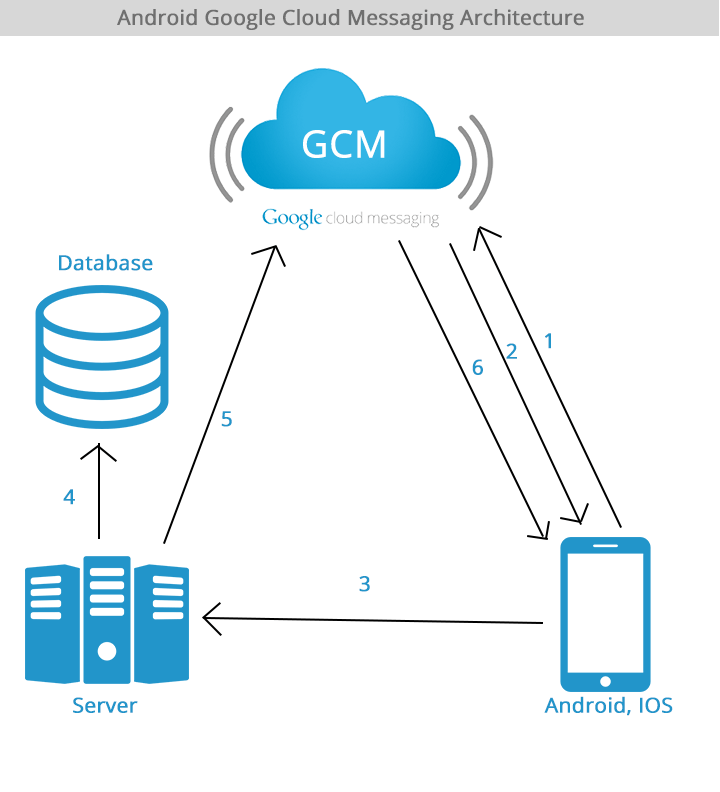
\includegraphics[height=200px]{push-notification-diagram.png}
  \caption{Fonctionnement des notifications push avec Firebase Cloud Messaging.}
  \label{fig:push_notification_fcm_explanation}
\end{figure}

Une étape supplémentaire est réalisée par le plugin Cordova. Ce dernier reçoit
la notification sous un format bien défini et construit la notification dans la
barre de notifications.

Le module \verb|Os_fcm_notif| implémente une interface OCaml simple pour
communiquer avec FCM en utilisant le plugin \emph{phonegap-plugin-fcm}.

Vincent Balat m'a ensuite demandé de créer une application mobile de test qui
servira plus tard de base à Be Sport.
Le projet est disponible sur GitHub \cite{ocsigen-mobile-push-notifications}. Il
est développé en utilisant une version modifiée du template d'Ocsigen Start qui
ne contient pas de base de données mais garde l'avantage du duo application
mobile - application web.

Cette démonstration permet d'envoyer différents types de notifications comme le
montre les figures \ref{fig:push_notification_example_application_web} et \ref{fig:push_example_notification_application_result}.

\begin{figure}
  \centering
  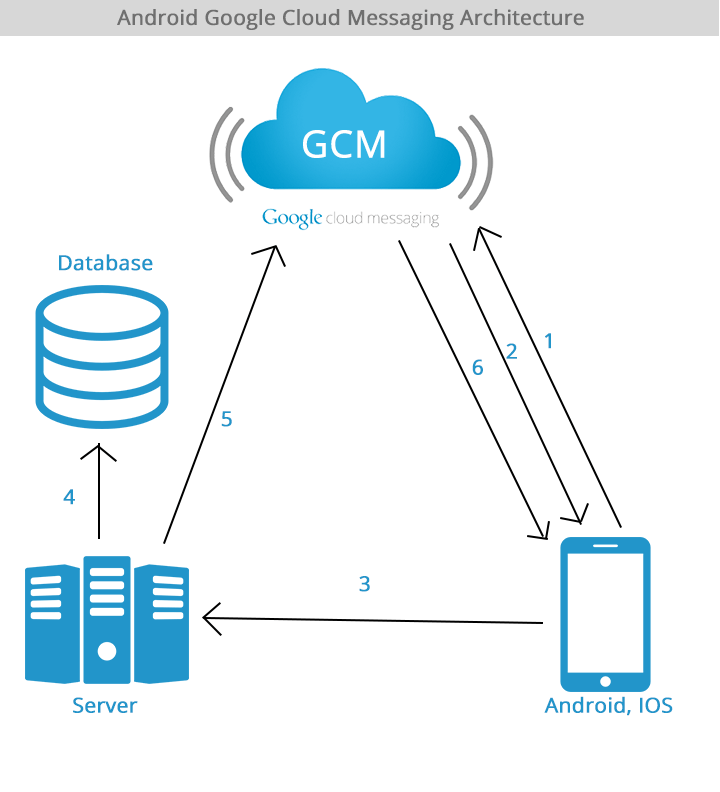
\includegraphics[height=200px]{push-notification-diagram.png}
  \caption{Exemple d'application montrant différents types de notifications push}
  \label{fig:push_notification_example_application_web}
\end{figure}

\begin{figure}
  \centering
  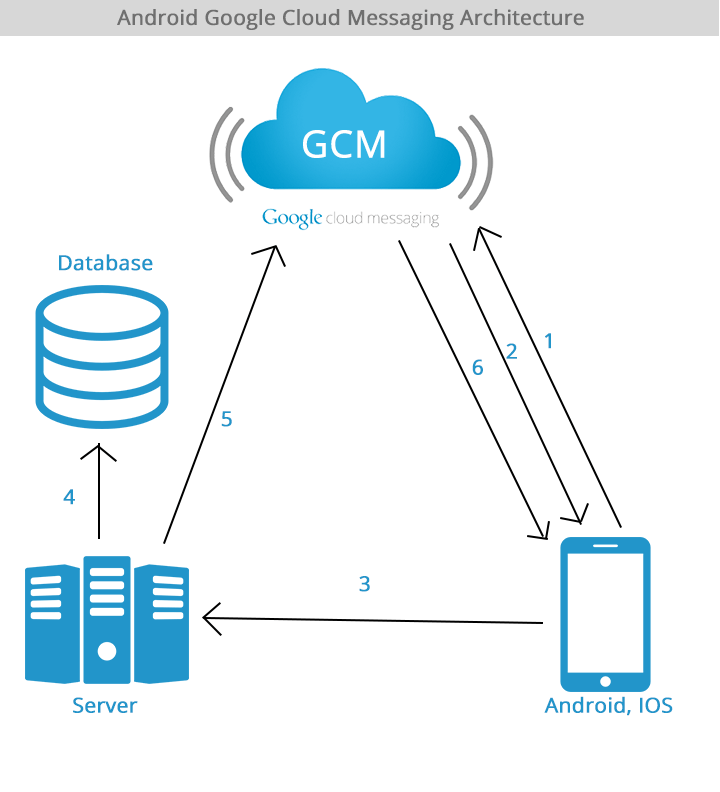
\includegraphics[height=200px]{push-notification-diagram.png}
  \caption{Notifications push reçu sur un smartphone Android.}
  \label{fig:push_notification_example_application_result}
\end{figure}

\subsubsection*{i18n}

\subsection{Personnelles}

A côté des heures passées dans les bureaux de Be Sport, j'ai continué à
m'intéresser au projet Ocsigen et à y contribuer. Bien que ces tâches soient
rapides, elles m'ont permis d'améliorer mes connaissances et d'être plus efficace
les jours suivants. Voici une liste non exhaustive:
\begin{itemize}
  \item eliom-distillery : option \verb|-list-templates| afin de lister tous les templates installés.
  \item eliom-distillery : option \verb|-y| pour ne pas demander de confirmation lors
    de la création d'un projet.
  \item eliom-distillery : options \verb|-add-git-template| et
\verb|-rm-template| pour permettre d'ajouter ses propres templates Eliom.\cite{eliom-distillery-repo}
  \item Binding OCaml au plugin Cordova
    \href{https://github.com/fechanique/cordova-plugin-fcm}{cordova-plugin-fcm}.\cite{ocaml-cordova-plugin-fcm} \\
    Celui-ci s'ajoute à la liste des bindings que j'ai réalisés pendant
l'année 2015-2016.\cite{ocaml-cordova-plugin-list}
\end{itemize}

\section{En dehors des tâches}

Mon stage ne m'a pas apporté que des connaissances techniques.

\subsection*{Be Sport}

Mon stage ne s'arrêtait pas aux différentes tâches décrites. Chaque semaine,
nous avions une réunion avec l'ensemble de l'équipe afin de faire le point sur
l'avancée de chaque fonctionnalité. Ces réunions m'ont permis d'être plus
ordonné et d'arriver à me positionner dans l'avancement d'une tâche.

La tâche des notifications push et d'OAuth2.0 et OpenID Connect m'ont permis de
travailler sur des fonctionnalités en partant d'une idée jusqu'à la réalisation
concrète en passant par la recherche et l'étude de solutions existantes et les
spécifications.

Pour certaines de mes tâches, j'ai été mené à travailler avec d'autres membres
de l'équipe qui n'étaient pas nécessairement développeurs (designers,
rédacteurs, etc). J'ai pu réaliser que discuter avec des personnes n'ayant pas
de compétences en développement nécessite un travail sur la forme et sur la vulgarisation des concepts.

\subsection*{Erasmus +}

La ville de mon lieu de stage n'était pas un choix anodin. Je souhaitais découvrir
Paris pour son ambiance entrepreneuriale et pour être au centre des évolutions
technologiques.
Régulièrement, je me suis rendu à des conférences ou des meetups pour
développeurs et entrepreneurs.

Pendant tout mon séjour à Paris, j'habitais dans une HackerHouse \cite{hackerhouse-website}, un espace de
coliving entre développeurs et entrepreneurs. Je vivais avec 8 autres personnes
partageant les mêmes passions et les mêmes ambitions que moi. Nous réalisions des événements autour du
développement ou de l'entrepreneuriat au moins 2 week-ends par mois. Cela m'a
permis d'agrandir mon réseau professionnel ainsi que mes connaissances.
Vivre avec d'autres entrepreneurs m'a permis de prendre conscience de la réalité
de l'entrepreneuriat et de compléter le cours d'entrepreneuriat que j'ai suivi
lors de ma première année de master à l'université de Mons.

\subsection*{Autres}

A partir de septembre, j'ai également eu la chance de pouvoir assister les
lundis matins à un cours donné à l'Ecole Normale Supérieure (\og
$\lambda$-calcul et catégories \fg). Cela m'a permis d'aborder les langages
fonctionnels et en particulier OCaml avec un aspect plus théorique et de faire
le lien avec l'algèbre et les catégories.

De plus, j'ai pu me rendre à une conférence donné par Richard Stallman. Cette
rencontre m'a permis de me sensibiliser encore plus aux licences et au monde du
libre.
\section{Conclusion}

J'ai également pu remarquer que les librairies ou technologies maintenues par de grandes
sociétés ne sont pas nécessairement meilleures ou les plus à jour. (exemple:
PhoneGap et phonegap-plugin-push ou Google et la documentation de FCM et l'API
de Google Maps).

Arrêter de considérer le tout comme une boite noire.

\nocite{*}

% Si vous utilisez (conseillé) BibTeX pour votre bibliographie :
\bibliographystyle{unsrt}
\bibliography{rapport-stage} % si le fichier BibTeX est rapport-stage.bib

\end{document}
%%% Local Variables: 
%%% mode: latex
%%% TeX-master: t
%%% TeX-PDF-mode: t
%%% End: 
